%%%%%%%%%%%%%%%%%%%%%%%%%%%%%%%%%%%%%%%%%%%%%%%%%%%%%%%%%%%%%%%%%%%%%%
% LaTeX Example: Project Report
%
% Source: http://www.howtotex.com
%
% Feel free to distribute this example, but please keep the referral
% to howtotex.com
% Date: March 2011
%
%%%%%%%%%%%%%%%%%%%%%%%%%%%%%%%%%%%%%%%%%%%%%%%%%%%%%%%%%%%%%%%%%%%%%%
% How to use writeLaTeX:
%
% You edit the source code here on the left, and the preview on the
% right shows you the result within a few seconds.
%
% Bookmark this page and share the URL with your co-authors. They can
% edit at the same time!
%
% You can upload figures, bibliographies, custom classes and
% styles using the files menu.
%
% If you're new to LaTeX, the wikibook is a great place to start:
% http://en.wikibooks.org/wiki/LaTeX
%
%%%%%%%%%%%%%%%%%%%%%%%%%%%%%%%%%%%%%%%%%%%%%%%%%%%%%%%%%%%%%%%%%%%%%%
% Edit the title below to update the display in My Documents
%\title{Project Report}
%
%%% Preamble
\documentclass[paper=a4, fontsize=12pt,DIV=14]{scrartcl}    % scrartcl = article-typed dcmt using pckg Koma-script
\usepackage[utf8]{inputenc}

\usepackage[english]{babel}							 % English language/hyphenation
\usepackage[protrusion=true,expansion=true]{microtype}
\usepackage[pdftex]{graphicx}	
\linespread{1}
\usepackage{array}
\usepackage{pdfpages}                               % Packages used to include pdf files
\usepackage{rotating}                               % Allow landscape mode for certain pages

%%% Custom sectioning
\usepackage{sectsty}
\allsectionsfont{\fontfamily{cmss}\selectfont}
\sectionfont{\sectionrule{3ex}{1pt}{-1.5ex}{1pt}}
\subsectionfont{\hspace*{2.5em}}
\paragraphfont{\hspace*{0.5em}}
\subsubsectionfont{\hspace*{5em}}

%%% Custom headers/footers (fancyhdr package)
\usepackage{fancyhdr}
\pagestyle{fancyplain}
\fancyhead[L]{R. Peree, G. Cartier}	% Left page header
\fancyhead[R]{
\includegraphics[scale=0.2]{img/logo.png}
\includegraphics[scale=0.2]{img/via_logo.png}}           % Right page header
\fancyfoot[L]{Autumn 2017}								        % Empty0
\fancyfoot[C]{}									            	% Empty
\fancyfoot[R]{\thepage}							            	% Page numbering
\renewcommand{\headrulewidth}{0pt}		                        % Remove header underlines
\renewcommand{\footrulewidth}{0pt}		                    	% Remove footer underlines
\setlength{\headheight}{20.4pt}
\setcounter{page}{-1}                                           % Starts the page numbering at -1


%%% Begin document
\begin{document}

	%\setlength{\parindent}{0cm}
%\setlength{\parskip}{1ex plus 0.5ex minus 0.2ex}
%\newcommand{\hsp}{\hspace{20pt}}
\newcommand{\HRule}{\rule{\linewidth}{0.5mm}}

\begin{titlepage}
  \begin{sffamily}
  \begin{center}

    
    % Upper part of the page. The '~' is needed because \\
    % only works if a paragraph has started.
    
\includegraphics[scale=0.7]{img/via_logo.png}~\\[1.5cm]

    \textsc{\Large Project Report }\\[1cm]

    % Title
    \HRule \\[0.4cm]
    { \huge \bfseries Surfing-couch\\[0.4cm] }

    \HRule \\[3cm]
    
\includegraphics[scale=0.75]{img/logo.png}\\[1.3cm]

    % Author and supervisor
    \begin{minipage}{0.35\textwidth}
      \begin{flushleft} \large
        Rosalie Peree \textsc{(258377)}\\
      \end{flushleft}
    \end{minipage}
    \begin{minipage}{0.35\textwidth}
      \begin{flushright} \large
        Grégoire Cartier \textsc{(258378)}\\
        %\emph{Chef d'équipe : } M. Chef \textsc{D’Équipe}
      \end{flushright}
    \end{minipage}\\[1.5cm]
    
    \Large\emph{Supervisor \& Academic advisor:} Kasper \& Jakob\textsc{}\\[1cm]


    \vfill

    % Bottom of the page
    {\large 2017 (Autumn semester)}
  \end{center}
  \end{sffamily}
\end{titlepage} %% Titlepage set in titlepage.tex
    \tableofcontents
    \thispagestyle{empty}           %used to remove the page number

    \newpage
        \section{Abstract}
        % COMPLETE SECTION TO DO
        % PROOF READ TO DO


    \newpage
        \section{Introduction}
        % COMPLETE SECTION TO DO
        % PROOF READ TO DO
        	\subsection{Background Description}
        	\subsection{Problem Description}
        	\subsection{Limitations and Delimitations}


    \newpage
        \section{Methods}
        % COMPLETE SECTION DONE
        % PROOF READ TO DO

	        \paragraph{}The following table presents our choice of model and methods for the problems that we listed in our project description (see Appendix \#1):
	        \paragraph{}

	        \begin{tabular}{|p{5cm}|p{5cm}|p{5.1cm}|}
	            \hline
                \textbf{What} \newline \textit{Problem} & \textbf{Why} \newline \textit{Why study this problem} & \textbf{Which} \newline \textit{Which models/theories did you use to solve the problem?}\\
                \hline
                \hline
                How can we develop a social application which is fun to use and rewards the user for helping travelers in their area? 
                & How to make the application interesting for our potential users?
                & We have to pay attention to all the following problems to be able to develop an application that will address all of them as good as possible.\\
                \hline
                What is important for travelers?
                & As our application is mainly targeted to travelers, it is interesting to know what is important for them, so that we cant try to implement those things in the final application.
                & We conducted a survey via Google Forms to gather people's opinion on that subject.\\
                \hline
                What is important for hosts?
                & As we want hosts to offer services to travelers, we have to meet with what they want to encourage them to do so.
                & We conducted a survey via Google Forms to gather potential user's opinion on that subject.\\
                \hline
                How can we allow users to create and find trips in their area and offer a service to travelers?
                & This problem is the main problem for a couch-surfing-like application. We have to localize the user to be able to provide a service for them in a specific area.
                & We have to set up a way for the users to enter their city/location and look for hosts in cities they want to visit.\\
                \hline
                How can we make the service secure for users?
                & Users don't want their personal data to be forwarded to strangers.
                & No personal data is displayed on the application for users to see. We implemented an internal messaging system so people can communicate directly on the application.\\
                \hline
                Can we add reviews and comments about travelers and hosts?
                & If you have to host someone or sleep/shower at a stranger's place, safety is very important. Users need a way to see if someone behaved correctly or not before their stay.
                & We implemented a system of user reviews - with grades - so people can report how they experience was with that specific user - hosts and travelers.\\
                \hline
            \end{tabular}

            \begin{tabular}{|p{5cm}|p{5cm}|p{5cm}|}
	            \hline
                \textbf{What} \newline Problem & \textbf{Why} \newline Why study this problem & \textbf{Which} \newline Which models/theories did you use to solve the problem?\\
                \hline
                \hline
                How can we define the point-value of the provided services?
                & As the system is based on a reward, all services must have a fixed value.
                & We defined a value for each service - sleep, shower and laundry. The points are given to the host once the booking is completed.\\
                \hline
                How can we exchange the points for gifts?
                & The system is based on rewarding hosts with gifts for providing a service.
                & We set up an online shop where users can exchange their points for goods.\\
                \hline
                How will the user interface be implemented?
                & The user interface has to be easy to get and use.
                & The interface will be an Android application.\\
                \hline
                What kind of tool will be used for this implementation?
                & The tools used to develop can make the process of developing the application more or less easy.
                & We decided to develop the application using Android Studio, as it is the platform we are both most familiar with.\\
                \hline
                How will the interface be user-friendly?
                & The interface has to be easy to use and understand for any user.
                & The interface is simple, with buttons and labels that are easy to understand. \\
                \hline
                How is the social interaction going to take place?
                &The point of the assignment is to enable a social interaction.
                & In our application, the social interaction will take place in the form of direct messaging between two users, a common chat for all the users and the possibility of reviewing experience with other users.\\
                \hline
                What kind of database will be implemented?
                & We need a database that is free and easy to integrate in Android.
                & The chosen database is Firebase for our project.\\
                \hline
            \end{tabular}


    \newpage
        \section{Requirements}
        % COMPLETE SECTION TO DO
        % PROOF READ TO DO
        	\paragraph{}The users of the application will be any person interested in traveling on a budget or having a different traveling experience, as well of any person that will be willing to host or provide a service -for now, shower and laundry - to a traveler visiting their city. They could be from everywhere in the world and have about any age, as long as they have access to a mobile phone running Android and a working Internet connection. They should not have an extensive knowledge of IT to be able to use the application.
        	\subsection{List of Requirements}
        		\subsubsection{Functional Requirements}
        			\paragraph{Use cases:}
        			\paragraph{}

		                \begin{figure}[!htbp]
		                    \center
		                    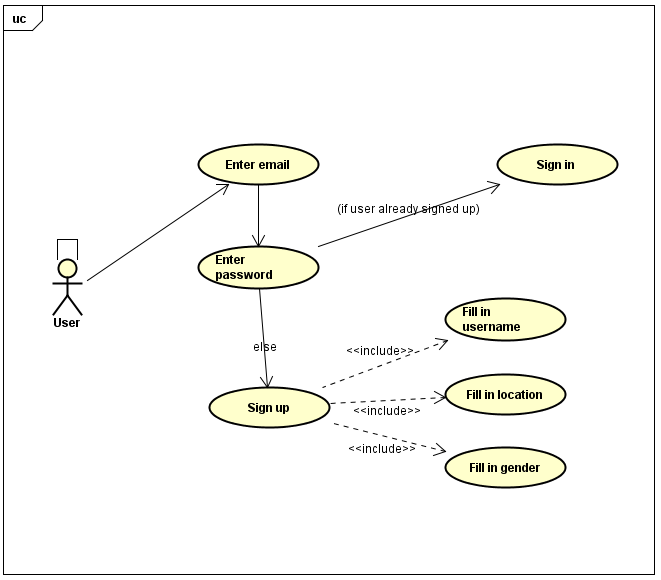
\includegraphics[scale=0.75]{img/enter_application.png}
		                    \caption{Use Case 1: how to access to application}
		                \end{figure}

		                \begin{figure}[!htbp]
		                    \center
		                    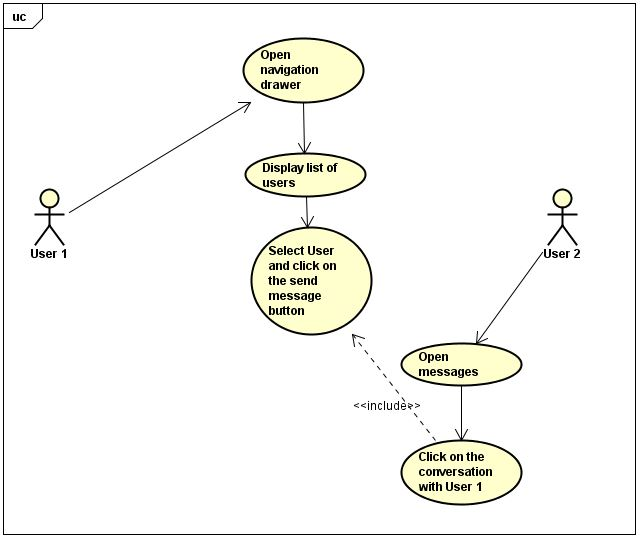
\includegraphics[scale=0.7]{img/send_message.png}
		                    \caption{Use Case 2: how users can communicate together by messages}
		                \end{figure}

		                \begin{figure}[!htbp]
		                    \center
		                    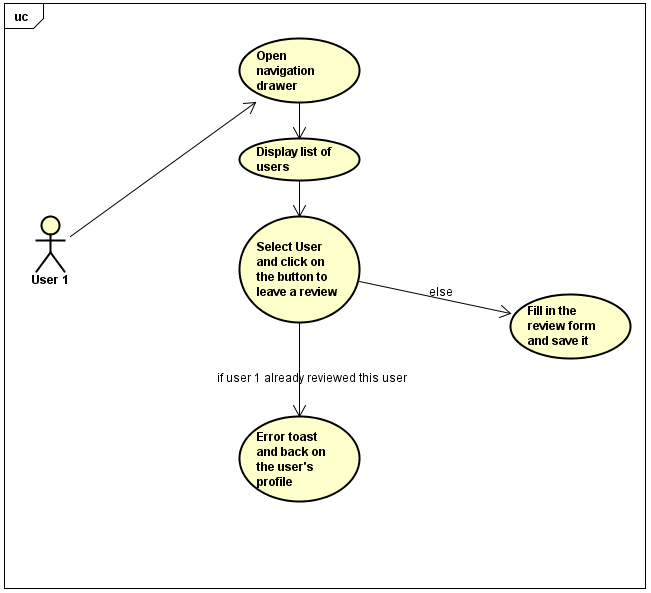
\includegraphics[scale=0.7]{img/leave_review.png}
		                    \caption{Use Case 3: how a user can leave a review to another user}
		                \end{figure}

		                \begin{figure}[!htbp]
		                    \center
		                    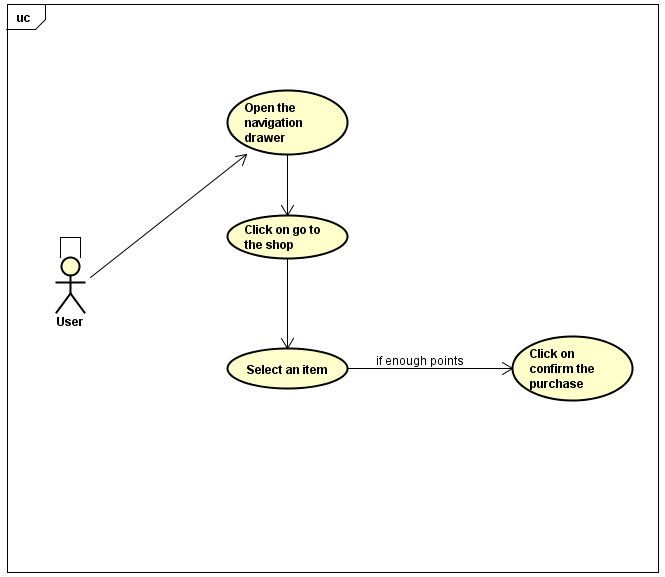
\includegraphics[scale=0.75]{img/shop.png}
		                    \caption{Use Case 4: how a user can cash his points for a reward}
		                \end{figure}

		                \paragraph{}

		                \paragraph{Activity Diagrams:}
        				\paragraph{}

		                \begin{figure}[!htbp]
		                    \center
		                    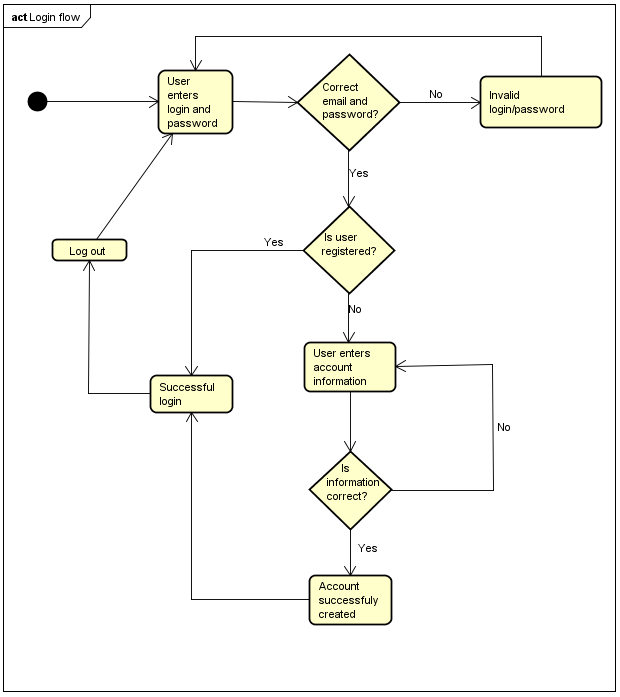
\includegraphics[scale=1]{img/act_login.png}
		                    \caption{Activity Diagram 1: sign in on the application}
		                \end{figure}
		                \newpage

		                \begin{figure}[!htbp]
		                    \center
		                    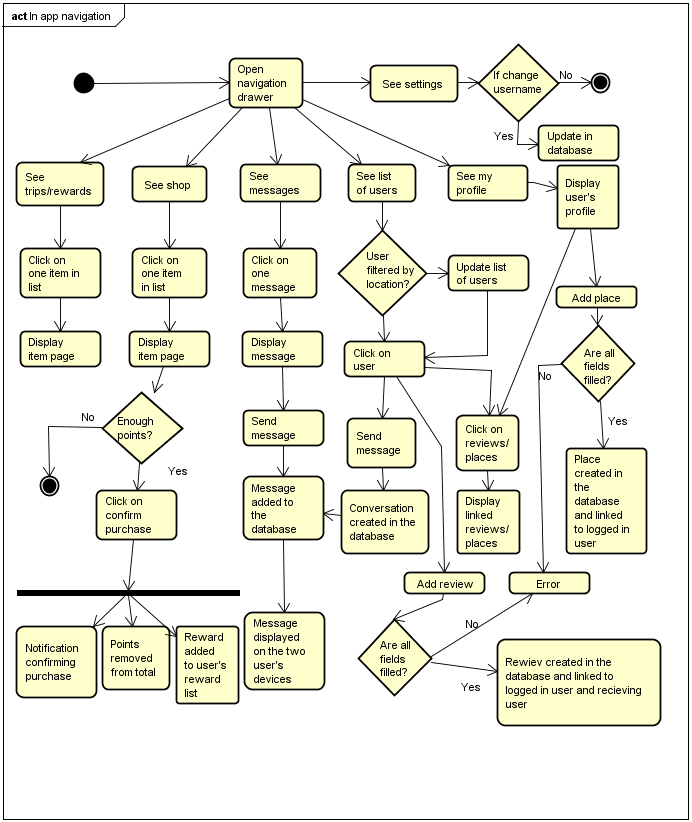
\includegraphics[scale=1]{img/act_navigation.png}
		                    \caption{Activity Diagram 2: navigation from the navigation drawer}
		                \end{figure}

		                \paragraph{}The second activity diagram groups some activities together. The activities that are merged together on the diagram are distinct activities, but have the same behavior and thus can be grouped together. This is done to avoid this diagram to become too complicated to read.

        		\subsubsection{Non-Functional Requirements}
        			\paragraph{Security}
        			\begin{itemize}
        				\item Password requirements (set up by Firebase)
        				\item Password security (hashed)
        				\item Password not saved unencrypted
        				\item If password lost, email to make a new one (handled by Firebase)
        			\end{itemize}
        			\paragraph{Usability}
        			\begin{itemize}
        				\item User friendly
        				\item Possible translation of the application due to avoiding hard-coded strings
        			\end{itemize}


    \newpage
        \section{Analysis}
        % COMPLETE SECTION TO DO
        % PROOF READ TO DO


    \newpage
        \section{Design}
        % COMPLETE SECTION TO DO
        % PROOF READ TO DO
        	\subsection{Architecture}
We used the Adapter in Android which is close to a Pattern Adapter.

\begin{figure}[!htbp]
							\center
		                    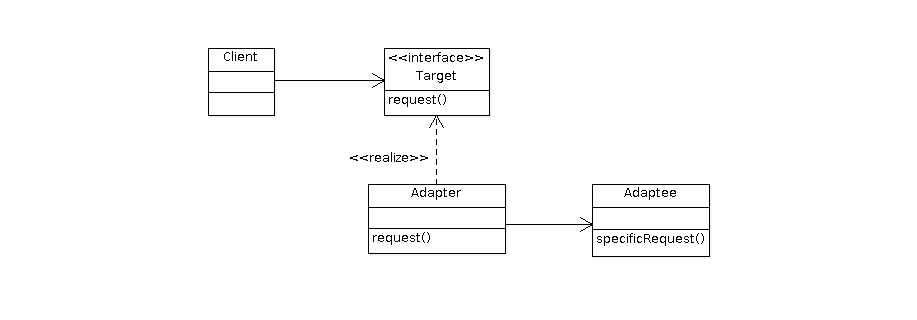
\includegraphics[scale=0.5]{img/adapterpattern.png}
		                    \caption{Adapter Pattern Template (\textit{softwarepassion.com})}
\end{figure}

We used those Adapters to populate the listViews with ArrayList and make clickable. Those Adapters are customizable, and help to display the content of the Objects that are kept in the database \\

We also wanted to use a MVC (Model View Controller), which is a MVP (Model View Presenter) but the scope of the project was too short to implement it correctly, and we didn't studied it during the Android course.



        	\newpage
        	\subsection{Technologies}
        		
\textbf{Surfing Couch} uses different technologies :\\
To do deal with all of the data manipulated by the users, the applications uses \textbf{Firebase} as database : \\
\begin{itemize}
\item Pros :
	\begin{itemize}
	\item 	Firebase provides an easy implementation on an Android application, there is not that much of a setup to do, the read and write functions are really easy to implement
	\item 	Firebase use JSON which permits an implementation of data in a fairly effortless way. That create a database that is flexible, well-structured and easy to read to some extent.
	\item 	Firebase gives useful tools, including a user authentication that deals with the security of database thanks to its data hashing. Firebase is also loaded with email confirmation, data analytics, and stability tools, which helps to make the user experience better.
	\item 	Made by Google
	\end{itemize}

\item Cons :
	\begin{itemize}
	\item	When the data structure starts to be a bit complex, it becomes quite hard to navigate through all of the data. Especially if you have a lot of data.
	\item	The querying and indexing is very limited due to the use of the JSON. It makes the search of data is very redundant.
	\item	Firebase is a bit high level, so you don’t feel you have that much of control over it
	\item	Made by Google
	\end{itemize}
\end{itemize}

One of the alternative to Firebase could be to use a more “classical” database management system like \textbf{SQLite} :
\begin{itemize}
\item Pros :
	\begin{itemize}
		\item	Classical way to store data, you can do SQL queries on it to retrieve data with more efficiency. Include also a good indexing of the data.
		\item	Is better than Firebase at storing huge load of data.
	\end{itemize}
\item Cons :
	\begin{itemize}
\item	You don’t have the tools proposed by Firebase, so you can really analyze your data usage and you must make all of the part of the security by yourself
\item	Harder to use and implement than Firebase.
	\end{itemize}
\end{itemize}

The application must be developed natively on Android, so \textbf{Android Studio} was a default choice to develop the application. But it's interesting to point out that there is alternatives to Android Studio such as \textbf{Xamarin} or \textbf{Cordova}.\\
\subsection{Design Patterns, Class Diagram, Sequence Diagrams}

Like said earlier, we are not using a specific design pattern.

\begin{figure}[!htbp]
							\center
		                    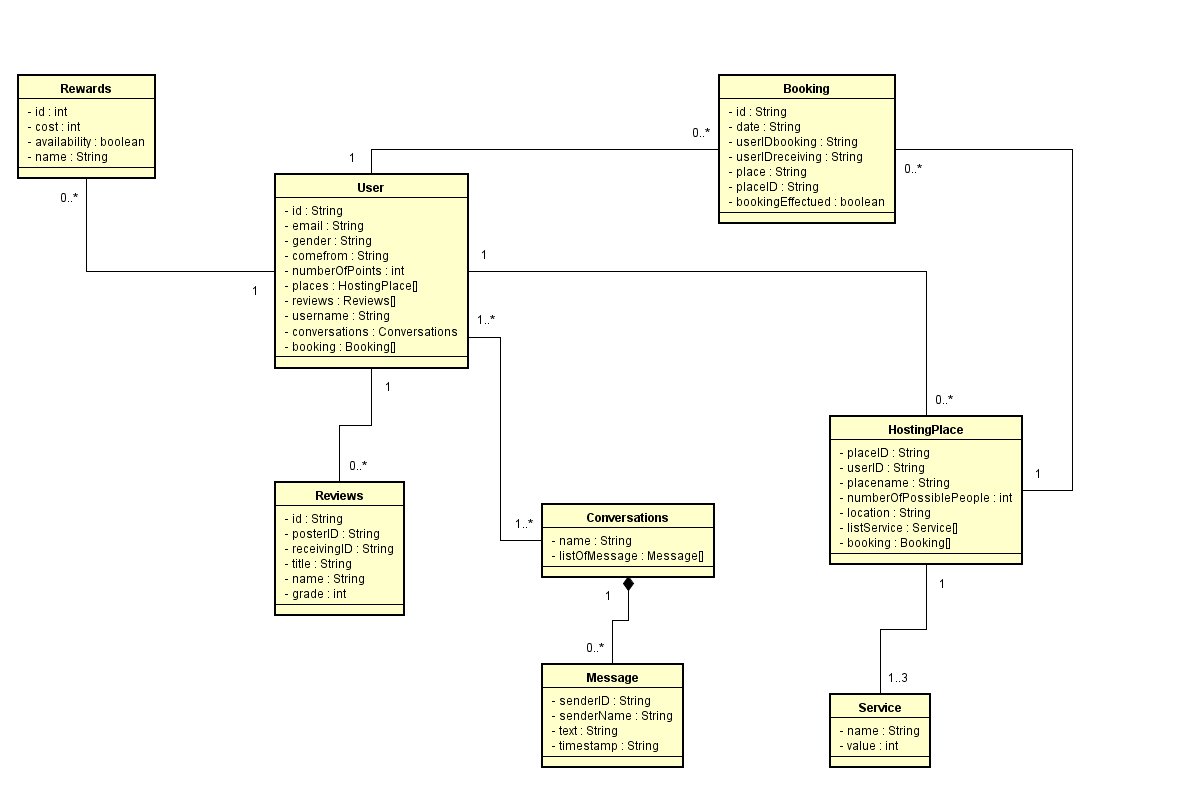
\includegraphics[scale=0.6]{img/class_diagram.png}
		                    \caption{Class Diagram of the database } 
\end{figure}

The database\footnote{We made a class diagram for the databse because the data is kept in a JSON} is pretty straightforward, everything is based around the User. However, we must highlight some details. By default, when a user is created, the bookings are null, so not present in the database JSON. The list is created with the first booking he makes.
Also, a default chat is assigned to each user which is the “General Chat” so can talk all together. The other List are defined as “undefined” and taken as HashMaps inside of the app.



\newpage


\begin{figure}[!htbp]
							\center
		                    \includegraphics[scale=0.5, angle = 90]{img/activity.png}
		                    \caption{Class Diagram of the Activities of the application} 

\end{figure}
\textit{See the annex file for better version}




    \newpage
        \section{Implementation}
        % COMPLETE SECTION TO DO
        % PROOF READ TO DO



    \newpage
        \section{Test}
        % COMPLETE SECTION TO DO
        % PROOF READ TO DO
        	\subsection{Test Specifications}
        	\subsection{White Box Testing}



    \newpage
        \section{Results \& Discussion}
        % COMPLETE SECTION TO DO
        % PROOF READ TO DO



    \newpage
        \section{Conclusion}
        % COMPLETE SECTION TO DO
        % PROOF READ TO DO


        %\newpage
\setlength{\parindent}{0cm}
\section{Sources, references and literature}
    \subsection{Definitely:}
        \begin{itemize}
%            % Marketing Bibliography
%            \item[] McDonald, Malcolm H.B. and Wilson, Hugh. 2016. \textit{Marketing plans: how to prepare them, how to use them.} Chichester: Wiley.
%            \item[] Belz, Frank-Martin and Peattie, Ken. 2009. \textit{Sustainability marketing: a global perspective.} Chichester: Wiley.
%            % ICT bibliography
%            \item[] Ford, J. (2009). \textit{Ajax programming for the absolute beginner.} 1st ed. Boston, MA: Course Technology Cengage Learning.
 %           \item[] Hazem, S. (2014). \textit{JavaScript Mobile Application Development.} 1st ed. Birmingham B3 2PB, UK.: Packt Publishing Ltd.
 %           \item[] Kumar Patel, S. (2014). \textit{Developing responsive web applications with AJAX and jQuery.} 1st ed. Birmingham, U.K: Packt Pub.
%            \item[] Montoro, A. (2011). \textit{IPhone JavaScript cookbook.} 1st ed. Birmingham, U.K.: Packt Pub.
 %           \item[] Shotts, K. (2014). \textit{PhoneGap 3.x Mobile Application Development Hotshot.} 1st ed. Birmingham: Packt Publishing.
%            \item[] Vohra, D. (2015). \textit{JavaServer Faces 2.0.} 1st ed.
%            \item[] Wagner, R. (2009). \textit{JavaScript \& Ajax for dummies.} 1st ed. New York: Wiley.
         \end{itemize}
    \subsection{Possibly:}
        \begin{itemize}
            % Marketing Bibliography
%            \item[] Comm, Joel and Taylor, David. 2015. \textit{Twitter power 3.0: how to dominate your market one tweet at a time.} Hoboken: Wiley.
%            \item[] Ruey-Jer Bryan Jean, Jyh-Shen Chiou and Shaoming Zou. 2013. \textit{International marketing in rapidly changing environments.} Bingley: Emerald.
%            \item[] Viardot, Eric. 2004. \textit{Successful marketing strategy for high-tech firms.} Boston: Artech House.
%            \item[] Shaoming Zou, Hui Xu and Linda Hui Shi. 2015. \textit{Entrepreneurship in international marketing.} Bingley: Emerald.
%            \item[] Stöttinger, Barbara, Schlegelmilch, Bodo B. and Zou, Shaoming. 2015. \textit{International marketing in the fast changing world.} Bingley: Emerald.
%            \item[] Chang, C.M. 2014. \textit{Business fundamentals for engineering managers.} New York: Momentum Press.
        \end{itemize}
\newpage                             % Adding the sources page

%%% End document
\end{document} 